%  A simple AAU report template.
%  2015-05-08 v. 1.2.0
%  Copyright 2010-2015 by Jesper Kjær Nielsen <jkn@es.aau.dk>
%
%  This is free software: you can redistribute it and/or modify
%  it under the terms of the GNU General Public License as published by
%  the Free Software Foundation, either version 3 of the License, or
%  (at your option) any later version.
%
%  This is distributed in the hope that it will be useful,
%  but WITHOUT ANY WARRANTY; without even the implied warranty of
%  MERCHANTABILITY or FITNESS FOR A PARTICULAR PURPOSE.  See the
%  GNU General Public License for more details.
%
%  You can find the GNU General Public License at <http://www.gnu.org/licenses/>.
%
%  A simple AAU report template.
%  2015-05-08 v. 1.2.0
%  Copyright 2010-2015 by Jesper Kjær Nielsen <jkn@es.aau.dk>
%
%  This is free software: you can redistribute it and/or modify
%  it under the terms of the GNU General Public License as published by
%  the Free Software Foundation, either version 3 of the License, or
%  (at your option) any later version.
%
%  This is distributed in the hope that it will be useful,
%  but WITHOUT ANY WARRANTY; without even the implied warranty of
%  MERCHANTABILITY or FITNESS FOR A PARTICULAR PURPOSE.  See the
%  GNU General Public License for more details.
%
%  You can find the GNU General Public License at <http://www.gnu.org/licenses/>.
%
\documentclass[11pt,twoside,a4paper,openright]{report}
%%%%%%%%%%%%%%%%%%%%%%%%%%%%%%%%%%%%%%%%%%%%%%%%
% Language, Encoding and Fonts
% http://en.wikibooks.org/wiki/LaTeX/Internationalization
%%%%%%%%%%%%%%%%%%%%%%%%%%%%%%%%%%%%%%%%%%%%%%%%
% Select encoding of your inputs. Depends on
% your operating system and its default input
% encoding. Typically, you should use
%   Linux  : utf8 (most modern Linux distributions)
%            latin1 
%   Windows: ansinew
%            latin1 (works in most cases)
%   Mac    : applemac
% Notice that you can manually change the input
% encoding of your files by selecting "save as"
% an select the desired input encoding. 
\usepackage[utf8]{inputenc}
% Make latex understand and use the typographic
% rules of the language used in the document.
\usepackage[danish,english]{babel}
% Use the palatino font
\usepackage[sc]{mathpazo}
\linespread{1.05}         % Palatino needs more leading (space between lines)
% Choose the font encoding
\usepackage[T1]{fontenc}
%%%%%%%%%%%%%%%%%%%%%%%%%%%%%%%%%%%%%%%%%%%%%%%%
% Graphics and Tables
% http://en.wikibooks.org/wiki/LaTeX/Importing_Graphics
% http://en.wikibooks.org/wiki/LaTeX/Tables
% http://en.wikibooks.org/wiki/LaTeX/Colors
%%%%%%%%%%%%%%%%%%%%%%%%%%%%%%%%%%%%%%%%%%%%%%%%
% load a colour package
\usepackage{xcolor}
\definecolor{aaublue}{RGB}{33,26,82}% dark blue
% The standard graphics inclusion package
\usepackage{graphicx}
% Set up how figure and table captions are displayed
\usepackage{caption}
\captionsetup{%
  font=footnotesize,% set font size to footnotesize
  labelfont=bf % bold label (e.g., Figure 3.2) font
}
% Make the standard latex tables look so much better
\usepackage{array,booktabs}
% Enable the use of frames around, e.g., theorems
% The framed package is used in the example environment
\usepackage{framed}

%%%%%%%%%%%%%%%%%%%%%%%%%%%%%%%%%%%%%%%%%%%%%%%%
% Mathematics
% http://en.wikibooks.org/wiki/LaTeX/Mathematics
%%%%%%%%%%%%%%%%%%%%%%%%%%%%%%%%%%%%%%%%%%%%%%%%
% Defines new environments such as equation,
% align and split 
\usepackage{amsmath}
% Adds new math symbols
\usepackage{amssymb}
% Use theorems in your document
% The ntheorem package is also used for the example environment
% When using thmmarks, amsmath must be an option as well. Otherwise \eqref doesn't work anymore.
\usepackage[framed,amsmath,thmmarks]{ntheorem}

%%%%%%%%%%%%%%%%%%%%%%%%%%%%%%%%%%%%%%%%%%%%%%%%
% Page Layout
% http://en.wikibooks.org/wiki/LaTeX/Page_Layout
%%%%%%%%%%%%%%%%%%%%%%%%%%%%%%%%%%%%%%%%%%%%%%%%
% Change margins, papersize, etc of the document
\usepackage[
  inner=28mm,% left margin on an odd page
  outer=41mm,% right margin on an odd page
  ]{geometry}
% Modify how \chapter, \section, etc. look
% The titlesec package is very configureable
\usepackage{titlesec}
\titleformat{\chapter}[display]{\normalfont\huge\bfseries}{\chaptertitlename\ \thechapter}{20pt}{\Huge}
\titleformat*{\section}{\normalfont\Large\bfseries}
\titleformat*{\subsection}{\normalfont\large\bfseries}
\titleformat*{\subsubsection}{\normalfont\normalsize\bfseries}
%\titleformat*{\paragraph}{\normalfont\normalsize\bfseries}
%\titleformat*{\subparagraph}{\normalfont\normalsize\bfseries}

% Clear empty pages between chapters
\let\origdoublepage\cleardoublepage
\newcommand{\clearemptydoublepage}{%
  \clearpage
  {\pagestyle{empty}\origdoublepage}%
}
\let\cleardoublepage\clearemptydoublepage

% Change the headers and footers
\usepackage{fancyhdr}
\pagestyle{fancy}
\fancyhf{} %delete everything
\renewcommand{\headrulewidth}{0pt} %remove the horizontal line in the header
\fancyhead[RE]{\small\nouppercase\leftmark} %even page - chapter title
\fancyhead[LO]{\small\nouppercase\rightmark} %uneven page - section title
\fancyhead[LE,RO]{\thepage} %page number on all pages
% Do not stretch the content of a page. Instead,
% insert white space at the bottom of the page
\raggedbottom
% Enable arithmetics with length. Useful when
% typesetting the layout.
\usepackage{calc}

%%%%%%%%%%%%%%%%%%%%%%%%%%%%%%%%%%%%%%%%%%%%%%%%
% Bibliography
% http://en.wikibooks.org/wiki/LaTeX/Bibliography_Management
%%%%%%%%%%%%%%%%%%%%%%%%%%%%%%%%%%%%%%%%%%%%%%%%
\usepackage[backend=bibtex,
  bibencoding=utf8
  ]{biblatex}
\addbibresource{bib/mybib}

%%%%%%%%%%%%%%%%%%%%%%%%%%%%%%%%%%%%%%%%%%%%%%%%
% Misc
%%%%%%%%%%%%%%%%%%%%%%%%%%%%%%%%%%%%%%%%%%%%%%%%
% Add bibliography and index to the table of
% contents
\usepackage[nottoc]{tocbibind}
% Add the command \pageref{LastPage} which refers to the
% page number of the last page
\usepackage{lastpage}
% Add todo notes in the margin of the document
\usepackage[
%  disable, %turn off todonotes
  colorinlistoftodos, %enable a coloured square in the list of todos
  textwidth=\marginparwidth, %set the width of the todonotes
  textsize=scriptsize, %size of the text in the todonotes
  ]{todonotes}

%%%%%%%%%%%%%%%%%%%%%%%%%%%%%%%%%%%%%%%%%%%%%%%%
% Hyperlinks
% http://en.wikibooks.org/wiki/LaTeX/Hyperlinks
%%%%%%%%%%%%%%%%%%%%%%%%%%%%%%%%%%%%%%%%%%%%%%%%
% Enable hyperlinks and insert info into the pdf
% file. Hypperref should be loaded as one of the 
% last packages
\usepackage{hyperref}
\hypersetup{%
	pdfpagelabels=true,%
	plainpages=false,%
	pdfauthor={Author(s)},%
	pdftitle={Title},%
	pdfsubject={Subject},%
	bookmarksnumbered=true,%
	colorlinks=false,%
	citecolor=black,%
	filecolor=black,%
	linkcolor=black,% you should probably change this to black before printing
	urlcolor=black,%
	pdfstartview=FitH%
}
% package inclusion and set up of the document
% see, e.g., http://en.wikibooks.org/wiki/LaTeX/Formatting#Hyphenation
% for more information on word hyphenation
\hyphenation{ex-am-ple hy-phen-a-tion short}
\hyphenation{long la-tex}% 
%  A simple AAU report template.
%  2015-05-08 v. 1.2.0
%  Copyright 2010-2015 by Jesper Kjær Nielsen <jkn@es.aau.dk>
%
%  This is free software: you can redistribute it and/or modify
%  it under the terms of the GNU General Public License as published by
%  the Free Software Foundation, either version 3 of the License, or
%  (at your option) any later version.
%
%  This is distributed in the hope that it will be useful,
%  but WITHOUT ANY WARRANTY; without even the implied warranty of
%  MERCHANTABILITY or FITNESS FOR A PARTICULAR PURPOSE.  See the
%  GNU General Public License for more details.
%
%  You can find the GNU General Public License at <http://www.gnu.org/licenses/>.
%
%
%
% see, e.g., http://en.wikibooks.org/wiki/LaTeX/Customizing_LaTeX#New_commands
% for more information on how to create macros

%%%%%%%%%%%%%%%%%%%%%%%%%%%%%%%%%%%%%%%%%%%%%%%%
% Macros for the titlepage
%%%%%%%%%%%%%%%%%%%%%%%%%%%%%%%%%%%%%%%%%%%%%%%%
%Creates the aau titlepage
\newcommand{\aautitlepage}[3]{%
  {
    %set up various length
    \ifx\titlepageleftcolumnwidth\undefined
      \newlength{\titlepageleftcolumnwidth}
      \newlength{\titlepagerightcolumnwidth}
    \fi
    \setlength{\titlepageleftcolumnwidth}{0.5\textwidth-\tabcolsep}
    \setlength{\titlepagerightcolumnwidth}{\textwidth-2\tabcolsep-\titlepageleftcolumnwidth}
    %create title page
    \thispagestyle{empty}
    \noindent%
    \begin{tabular}{@{}ll@{}}
      \parbox{\titlepageleftcolumnwidth}{
        \iflanguage{danish}{%
          
\includegraphics[width=\titlepageleftcolumnwidth]{figures/aau_logo_da}
        }{%
          
\includegraphics[width=\titlepageleftcolumnwidth]{figures/aau_logo_en}
        }
      } &
      \parbox{\titlepagerightcolumnwidth}{\raggedleft\sf\small
        #2
      }\bigskip\\
       #1 &
      \parbox[t]{\titlepagerightcolumnwidth}{%
      \textbf{Abstract:}\bigskip\par
        \fbox{\parbox{\titlepagerightcolumnwidth-2\fboxsep-2\fboxrule}{%
          #3
        }}
      }\\
    \end{tabular}
    \vfill
    \iflanguage{danish}{%
      \noindent{\footnotesize\emph{Rapportens indhold er frit tilgængeligt, men offentliggørelse (med kildeangivelse) må kun ske efter aftale med forfatterne.}}
    }{%
      \noindent{\footnotesize\emph{The content of this report is freely available, but publication (with reference) may only be pursued due to agreement with the author.}}
    }
    \clearpage
  }
}

%Create english project info
\newcommand{\englishprojectinfo}[8]{%
  \parbox[t]{\titlepageleftcolumnwidth}{
    \textbf{Title:}\\ #1\bigskip\par
    \textbf{Theme:}\\ #2\bigskip\par
    \textbf{Project Period:}\\ #3\bigskip\par
    \textbf{Project Group:}\\ #4\bigskip\par
    \textbf{Participant(s):}\\ #5\bigskip\par
    \textbf{Supervisor(s):}\\ #6\bigskip\par
    \textbf{Copies:} #7\bigskip\par
    \textbf{Page Numbers:} \pageref{LastPage}\bigskip\par
    \textbf{Date of Completion:}\\ #8
  }
}

%Create danish project info
\newcommand{\danishprojectinfo}[8]{%
  \parbox[t]{\titlepageleftcolumnwidth}{
    \textbf{Titel:}\\ #1\bigskip\par
    \textbf{Tema:}\\ #2\bigskip\par
    \textbf{Projektperiode:}\\ #3\bigskip\par
    \textbf{Projektgruppe:}\\ #4\bigskip\par
    \textbf{Deltager(e):}\\ #5\bigskip\par
    \textbf{Vejleder(e):}\\ #6\bigskip\par
    \textbf{Oplagstal:} #7\bigskip\par
    \textbf{Sidetal:} \pageref{LastPage}\bigskip\par
    \textbf{Afleveringsdato:}\\ #8
  }
}

%%%%%%%%%%%%%%%%%%%%%%%%%%%%%%%%%%%%%%%%%%%%%%%%
% An example environment
%%%%%%%%%%%%%%%%%%%%%%%%%%%%%%%%%%%%%%%%%%%%%%%%
\theoremheaderfont{\normalfont\bfseries}
\theorembodyfont{\normalfont}
\theoremstyle{break}
\def\theoremframecommand{{\color{gray!50}\vrule width 5pt \hspace{5pt}}}
\newshadedtheorem{exa}{Example}[chapter]
\newenvironment{example}[1]{%
		\begin{exa}[#1]
}{%
		\end{exa}
}
% my new macros

\begin{document}
%frontmatter
\pagestyle{empty} %disable headers and footers
\pagenumbering{roman} %use roman page numbering in the frontmatter
%  A simple AAU report template.
%  2015-05-08 v. 1.2.0
%  Copyright 2010-2015 by Jesper Kjær Nielsen <jkn@es.aau.dk>
%
%  This is free software: you can redistribute it and/or modify
%  it under the terms of the GNU General Public License as published by
%  the Free Software Foundation, either version 3 of the License, or
%  (at your option) any later version.
%
%  This is distributed in the hope that it will be useful,
%  but WITHOUT ANY WARRANTY; without even the implied warranty of
%  MERCHANTABILITY or FITNESS FOR A PARTICULAR PURPOSE.  See the
%  GNU General Public License for more details.
%
%  You can find the GNU General Public License at <http://www.gnu.org/licenses/>.
%
\pdfbookmark[0]{Front page}{label:frontpage}%
\begin{titlepage}
  \addtolength{\hoffset}{0.5\evensidemargin-0.5\oddsidemargin} %set equal margins on the frontpage - remove this line if you want default margins
  \noindent%
  \begin{tabular}{@{}p{\textwidth}@{}}
    \toprule[2pt]
    \midrule
    \vspace{0.2cm}
    \begin{center}
    \Huge{\textbf{
      Double tracking antennas for drone communication% insert your title here
    }}
    \end{center}
    \begin{center}
      \Large{
        - Automation and control -% insert your subtitle here
      }
    \end{center}
    \vspace{0.2cm}\\
    \midrule
    \toprule[2pt]
  \end{tabular}
  \vspace{4 cm}
  \begin{center}
    {\large
      Project Report%Insert document type (e.g., Project Report)
    }\\
    \vspace{0.2cm}
    {\Large
      Group 832%Insert your group name or real names here
    }
  \end{center}
  \vfill
  \begin{center}
  Aalborg University\\
  Electronics and IT
  \end{center}
\end{titlepage}
\clearpage
\thispagestyle{empty}
{\small
\strut\vfill % push the content to the bottom of the page
\noindent Copyright \copyright{} Aalborg University 2015\par
\vspace{0.2cm}
\noindent Here you can write something about which tools and software you have used for typesetting the document, running simulations and creating figures. If you do not know what to write, either leave this page blank or have a look at the colophon in some of your books.
}
\clearpage
\pdfbookmark[0]{English title page}{label:titlepage_en}
\aautitlepage{%
  \englishprojectinfo{
    Double Tracking Antennas for \\
    UAS Communication %title
  }{%
    Multivariable Control %theme
  }{%
    Spring Semester 2016 %project period
  }{%
    CA832 % project group
  }{%
    %list of group members
    Alvaro Perez Ortega\\ 
    Kenny Lund Lafon\\
    Kelvin Kjærvik Pagels\\
    Robert-Octavian Popescu\\
    Orlando Bastos Vaz
  }{%
    %list of supervisors
    Anders La Cour Harbo
  }{%
    1 % number of printed copies
  }{%
    \today % date of completion
  }%
}{%department and address
  \textbf{Electronics and IT}\\
  Aalborg University\\
  \href{http://www.aau.dk}{http://www.aau.dk}
}{% the abstract
  In an Unamanned Aircraft System (UAS) scenario, one of the main goals is to secure Line-of-Sight (LOS) between the Unmanned Aicraft (UA) and the Ground Station (GS). Moreover, in most cases permanent communication between systems must be assured. Such that, tracking directional antennas in both ends have been considered to have assure this communication. 

  Furthermore, the tracking is done with the help of a DC servomotor which will turn each antenna. Additionally, different controller's have been tested and tunned for this specific application to achieve valuable results. Also, 2D and 3D simulations of the whole system have been made with the servomotor model and controller integrated.  
  
  The scope of the tracking is to achieve satisfactory link budget over long distances. In such a way, large areas can be covered in any application that requires permanent communication between GS and UA. 
}

\cleardoublepage
% {\selectlanguage{danish}
% \pdfbookmark[0]{Danish title page}{label:titlepage_da}
% \aautitlepage{%
%   \danishprojectinfo{
%     Double tracking antennas for drone communication %title
%   }{%
%     Multivariable control %theme
%   }{%
%     Spring 2016 %project period
%   }{%
%     Group: 832 % project group
%   }{%
%     %list of group members
%     Alvaro Perez Ortega\\ 
%     Kenny Lund Lafon\\
%     Kelvin Kjærvik Pagels\\
%     Robert-Octavian Popescu\\
%     Orlando Vaz
%   }{%
%     %list of supervisors
%     Anders La Cour Harbo
%   }{%
%     1 % number of printed copies
%   }{%
%     \today % date of completion
%   }%
% }{%department and address
%   \textbf{Elektronik og IT}\\
%   Aalborg Universitet\\
%   \href{http://www.aau.dk}{http://www.aau.dk}
% }{% the abstract
%   Her er resuméet
% }}
\cleardoublepage
\pdfbookmark[0]{Contents}{label:contents}
\pagestyle{fancy} %enable headers and footers again
\tableofcontents
\listoftodos
\chapter*{Preface\markboth{Preface}{Preface}}\label{ch:preface}
\addcontentsline{toc}{chapter}{Preface}
Here is the preface. You should put your signatures at the end of the preface.

\vspace{\baselineskip}\hfill Aalborg University, \today
\vfill\noindent
\begin{minipage}[b]{0.45\textwidth}
 \centering
 \rule{\textwidth}{0.5pt}\\
  Alvaro Perez Ortega\\
 {\footnotesize <aperez15@student.aau.dk>}
\end{minipage}
\hfill
\begin{minipage}[b]{0.45\textwidth}
 \centering
 \rule{\textwidth}{0.5pt}\\
  Kelvin Kjærvik Pagels\\
 {\footnotesize <kpagel15@student.aau.dk>}
\end{minipage}

\vspace{3\baselineskip}
\noindent
\begin{minipage}[b]{0.45\textwidth}
 \centering
 \rule{\textwidth}{0.5pt}\\
  Kenny Lund Lafon\\
 {\footnotesize <klafon15@student.aau.dk>}
\end{minipage}
\hfill
\begin{minipage}[b]{0.45\textwidth}
 \centering
 \rule{\textwidth}{0.5pt}\\
  Orlando Vaz\\
 {\footnotesize <obasto16@student.aau.dk>}
\end{minipage}

\vspace{3\baselineskip}

\begin{center}
\begin{minipage}[b]{0.45\textwidth}
 \centering
 \rule{\textwidth}{0.5pt}
  Robert-Octavian Popescu\\
 {\footnotesize <rpopes15@student.aau.dk>}
\end{minipage}
\end{center}

\cleardoublepage
%mainmatter
\pagenumbering{arabic} %use arabic page numbering in the mainmatter
\chapter{Worksheet 1 - February 10th \\ Scenario}\label{ch:WS1}
\section{Problem: Forest fire}
Wildfires in some countries can be a huge problem. Devastating forests, plantations or even habitations, the causes of such fires can be natural or criminal.
Each year wildfires destroy 6 to 14 million hectares of fire-sensitive forests worldwide. Throughout the world, forest fires are out of control. As an example at least one hundred villages are burned every year in Nepal, and some of them are destroyed by forest fires.
In order to prevent these catastrophes, fire lookout towers, public hotlines, ground and aerial patrols are used to detect fire starts. However, this surveillance has to be done day and night in large areas, resulting in high costs and risks for the patrols.

\section{Solution: Drone surveillance}
Early location and identification of fires is needed. A solution to improve the actual surveillance could be the use drones in order to fly long distances and cover large areas to find forest fires in an incipient stage. Also, this will minimize risks and time spent on such operations. 

\subsection{Project Scope}
\begin{itemize}  
        \item Assure permanent connection between drone and GNS
        \item Use directional antennas for both drone and GNS 
        \item Control both antennas to have maximum directivity (pointing directly at each other)
\end{itemize}

\subsection{Constraints}
\begin{itemize}  
        \item Limited frequency and bandwidth by means of the Law
        \item Limited antenna power and size
\end{itemize}

\subsection{Scenario parameters}
We assume that the risk area that the drone will cover is a rectangle:
\begin{equation*}\label{eq:scenario_parameters1} 
 		A_{zone} = xy
\end{equation*}

\begin{figure}[hb]
  	\centering
 	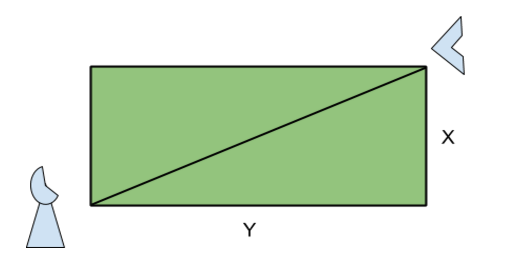
\includegraphics[width=0.8\textwidth]{figures/pic1.png}
  	\caption[Pipeline survey]{Scenario}
\end{figure}

Given the area of the rectangle we can compute the maximum distances of communication, which is the diagonal of the rectangle: 
\begin{equation*}\label{eq:scenario_parameters2} 
 		d_{max} = \sqrt{x^2 + y^2}
\end{equation*}
This distance will be taken into account when computing the radio link communication between the drone and GNS.

\section{Link Budget}\label{subsec:link_budget}
\paragraph{}
As the next step, once it is assured that there is Line-Of-Sight connection, it is important to calculate what is termed as the \textbf{Link budget}. This calculation is an accounting of all the gains and losses from the transmitter, through the medium,  to the receiver in a telecommunication system. It includes terms on it for the attenuation of the transmitted signal due to propagation, as well as the antenna gains, feedline and miscellaneous losses. It is precesily by assesing the link budget that is possible to design the system so that it meets the requirements and performs as desired. Its general form is:
\begin{equation*}\label{eq:link_budget} 
 		\text{Received Power (dBm)} = \text{Transmitted Power (dBm)} + \text{Gains (dB)} - \text{Losses(dB)}
\end{equation*}

And, in a more detailed look, it can divided down into:

\begin{equation*}\label{eq:link_budget} 
 		P_{RX} = P_{TX} + G_{TX} - L_{TX} - L_{FS} - L_{M} + G_{RX} - L_{RX}
\end{equation*}
where,
\begin{itemize}
\item{$P_{RX} -$ Recieved power [dBm]}
\item{$P_{TX} -$ Transmitter output power [dBm]}
\item{$G_{TX} -$ Transmitter antenna gain [dBi]}
\item{$L_{TX} -$ Transmitter feeder and associated losses (transmission line, connectors, etc.) [dB]}
\item{$L_{FS} -$ \textbf{Free Space Loss} or \textbf{Path Loss} [dB]}
\item{$L_{M} -$ Miscellaneus signal propagation losses (fading margin, polarization mismatch, other losses...) [dB]} 
\item{$G_{RX} -$ Receiver Antenna Gain [dBi]}
\item{$L_{RX} -$ Receiver feeder and associated losses (transmission line, connectors, etc.) [dB]} 
\end{itemize}
Note that losses are treated as possitive numbers and therefore they appear as a substraction in the link budget. Also highlight that decibels are logarithmic measurements, so adding decibels is equivalent to multiplying the actual numeric ratios.
 
\subsection{Free Space Loss}\label{subsec:path_loss}
\paragraph{}
The free space path loss is the loss in signal strength that occurs when an electromagnetic wave travels over a line of sight path in free space. In these circumstances there are no obstacles that might cause the signal to be reflected, refracted, or that might cause additional attenuation. Equation \ref{eq:path_losses} represents the loss in signal strength in dB.

\begin{equation}\label{eq:path_losses}
	L_{FS}\text{ [dB]} = 20\log\left (\frac{4\pi d}{\lambda} \right)
\end{equation}
where
\begin{itemize}
	\item d - Distance from transmitter to receiver [m]
	\item $\lambda  = \dfrac{c}{f} = \frac{\text{speed of light [m/s]}}{\text{frequency [Hz]}}$ - wavelength of the signal [m]
\end{itemize}

\paragraph{} Note then that a larger distance value between GS and UAV will result in higher path loss.

\subsection*{Effect of multipath propagation}
\paragraph{}For true free space propagation such as that encountered for satellites there will be no noticeable reflections and there will only be one major path. However for terrestrial systems, the signal may reach the receiver via a number of different paths as a result of reflections, etc that will occur as a result of the objects around the path. Buildings, trees, objects around the office and home can all cause reflections that will result in the signal variations.

\paragraph{}The multipath propagation will cause variations of the signal strength when compared to that calculated from the free space path loss. If the signals arrive in phase with the direct signal, then the reflected signals will tend to reinforce the direct signal. If they are out of phase, then they will tend to cancel the signal. If either the transmitter or receiver moves, then the signal strength will be seen to vary as the relative strengths and phases of the different signals change.
\chapter{Path loss}\label{ch:path_loss}

The free space path loss (FSPL) is the loss in signal strength that occurs when an electromagnetic wave travels over a line of sight path in free space. In these circumstances there are no obstacles that might cause the signal to be reflected, refracted, or that might cause additional attenuation. Equation \ref{eq:path_losses} represents the loss in signal strength.

\begin{equation}\label{eq:path_losses}
L = 20log\left (\frac{4\pi d}{\lambda} \right)
\end{equation}

The wave length can also be described by a relationship between the frequency and the velocity which is the light speed because radio waves are electromagnetic waves. This relationship is described by the equation \ref{eq:vel_freq_wavelen1}.

\begin{equation}\label{eq:vel_freq_wavelen1}
\lambda = \frac{c}{f}
\end{equation}


Explanation of the parameters.
\begin{itemize}
\item d - distance from transmitter to receiver [m]
\item $\lambda$ - wavelength of the signal [m]
\item c - speed of light constant $3\cdot 10^8$ [m/s] 
\item f - frequency of signal [Hz]
\end{itemize}

Consider our scenario we will assume that the distance is the maximum communication distance between the base station and the UAV. 
\begin{equation*}
Assume \begin{cases}
d = max\{ d_{com} \} = \sqrt{x^2+y^2} \text{km}\\
\text{f} = \text{MHz (Permitted frequency by law})\\
\end{cases}
\end{equation*}

Computing our signal wavelength:
\begin{equation}\label{eq:vel_freq_wavelen2}
\lambda = \frac{c}{f} = \frac{3\times 10^{8}}{f\times 10^{6}}=\frac{300}{f}=\frac{3}{10f}m
\end{equation}

Computing the path loss:
\begin{align*}\label{eq:path_loses_calc}
L = 20log\left (\frac{4\pi d}{\lambda} \right) dB &= 20log\left (\frac{4\pi \sqrt{x^2+y^2}}{\frac{3}{10f}} \right) dB \\ 
&= 20log\left (\frac{4\pi \sqrt{x^2+y^2}\cdot 10f}{ 3} \right) dB
\end{align*}

\noindent \textbf{As an observation, higher distance value between basestation and UAV will result in higher path loss.}
\subsection*{Line-Of-Sight Propagation}
\paragraph{}
At low frequency (below approximately 3 MHz) radio signals travel as ground waves, which follow the Earth's curvature due to diffraction with the layers of the atmosphere.
However, at higher frequencies and in lower levels of the atmosphere, neither of these effects are significant. Thus any obstruction between the transmitting antenna (transmitter) and the receiving antenna (receiver) will block the signal, just like the light that the eye may sense. Therefore, since the ability to visually see a transmitting antenna (disregarding the limitations of the eye's resolution) roughly corresponds to the ability to receive a radio signal from it, the propagation characteristic of VHF and higher radio frequency (>30 MHz) paths is called line-of-sight. The farthest possible point of propagation is referred to as the radio horizon.

The radio horizon is the locus of points at which direct rays from an antenna are tangential to the surface of the Earth. If the Earth were a perfect sphere and there were no atmosphere, the radio horizon would be a circle.

This way the greatest distance at which a receiver can see the transmiter is explained in the following figure:
\begin{equation*}\label{eq:link_budget} 
 		\text{Received Power (dBm)} = \text{Transmitted Power (dBm)} + \text{Gains (dB)} - \text{Losses(dB)}
\end{equation*}

In more detailed a common radio link looks like this:

\begin{equation*}\label{eq:link_budget} 
 		P_{RX} = P_{TX} + G_{TX} - L_{TX} - L_{FS} - L_{M} + G_{RX} - L_{RX}
\end{equation*}

Note that decibels are logarithmic measurements, so adding decibels is equivalent to multiplying the actual numeric ratios.
\begin{figure}[hb]
  	\centering
 	
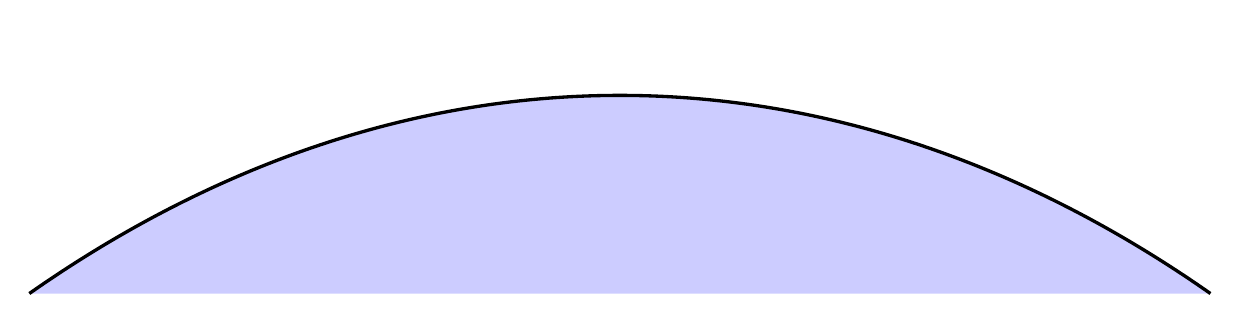
\begin{tikzpicture}
\draw[very thick, draw=black, fill=blue, fill opacity=0.2] (0,0) to [out=35,in=145] (15,0);
\end{tikzpicture}
  	\caption[Pipeline survey]{Scenario}
\end{figure}

\section*{Unmanned Aerial System (UAS)}
In some cases it is necessary to talk about our system as a whole, such that we use it further. The UAS is composed of the following:
\begin{itemize}
	\item Drone
	\item Basestation
	\item Communications
	\item Survey camera
\end{itemize}

\begin{figure}[h!]\label{fig:uas}
	\centering
	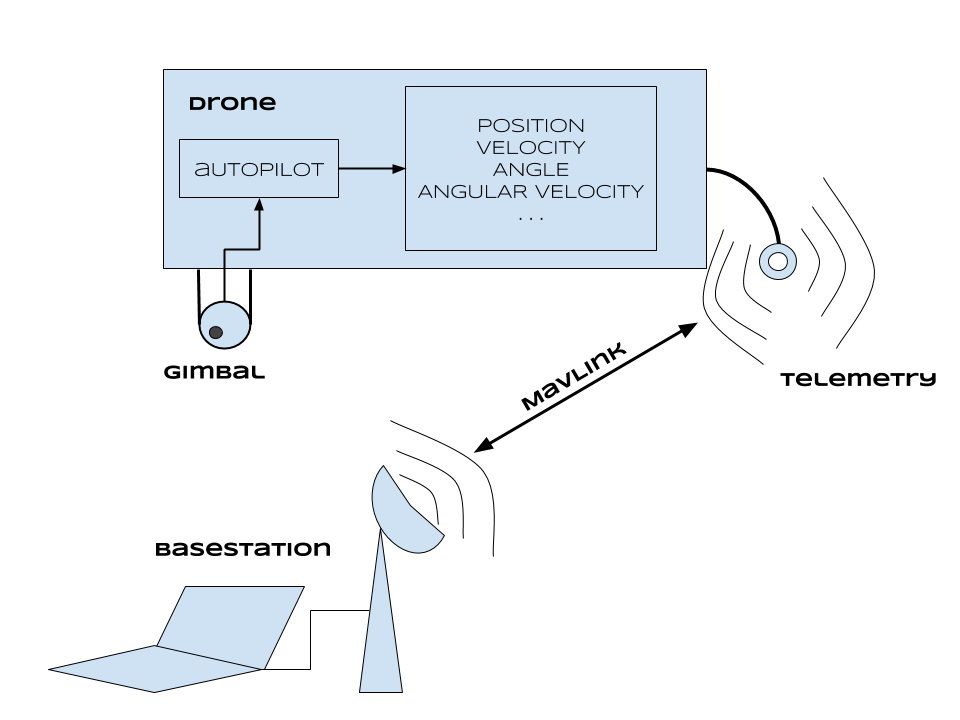
\includegraphics[width=0.7\textwidth]{figures/uas.png}
	\caption{Unmanned Aerial System Overview}
\end{figure}

\section*{Antenna Overview}
The antennas used for the basestation and the drone are different by means of weight and size. The preference of using them is based on the application at hand, thus for:
\begin{itemize}
	\item Basestation - Parabolic (grid) directional antenna 
	\item Drone - Patch directional antenna
\end{itemize}

A parabolic antenna in an antenna that uses a parabolic reflector and a curved surface to direct the radio waves and its main advantage is that it has a high directivity. This type of antennas are able to produce the narrowest beam widths which allow them to have some of the highest gains.

Parabolic antennas, due to their high gain, are intensively used for carry telephone and television signals between nearby cities. In our specific case, it’s possible to use this property to receive the information provided by the thermal camera through the UAS.

Patch antenna, which is the original type of microstrip, is a low profile antenna that can be mounted on a flat surface and it consists in a rectangular sheet of metal. These antennas are very useful because they are very thin and their directivity varies from 5 to 7 dB.

\begin{table}[h!]
\centering
	\begin{tabular}{|c||c|c|}
		\hline
		Parameter & Basestation & Drone\\ \hline\hline
		Type & Parabolic & Patch\\ \hline
		Polarization & Linear & Linear\\ \hline
		Frequency [GHz] & $2.4$ & $2.4$\\ \hline
		Gain [dB] & $24$ & $14$\\ \hline
		HPBW/$H(^{\circ})$ & $14$ & $45$\\ \hline
		HPBW/$V(^{\circ})$ & $10$ & $45$\\ \hline
	\end{tabular}
	\caption{Table of antennas parameters}
	\label{table:1}
\end{table}

\section*{Technical Scenario}
As mentioned before we need to assure the maximum distance of communication possible between the basestation and the drone at a certain working frequency:

\begin{equation*}\label{eq:tech_parameters1} 
 	\begin{cases}
 		d_{max} = 50 km	\\
 		f = 2.4 GHz
 	\end{cases}
\end{equation*}

Computing signal wavelength ($\lambda$) for the working frequency stated above:
\begin{equation*}\label{eq:tech_parameters2}
	\lambda = \frac{c}{f} = \frac{3\cdot 10^{8}}{2.4\cdot 10^{9}} 
	        = 0.125 \text{m}
\end{equation*}

Computing the path loss for a distance of 50 kilometers and the signal wavelength:
\begin{equation*}\label{eq:tech_parameters3}
	L = 20\lg\left (\frac{4\pi d_{max}}{\lambda} \right)
	  = 20\lg\left (\frac{4\pi \cdot 50}{0.125\cdot 10^{-3}} \right)
	  = 134 \text{dB} 
\end{equation*}


Computing the output power of the transmitting antenna of 1 Watt:
\begin{equation*}\label{eq:tech_parameters4}
	P_{TX} = 10\lg\left (\frac{1}{10^{-3}} \right)  
	       = 30 \text{dBm}
\end{equation*}


A simplified link budget omitting some losses of the UAS:
\begin{equation*}\label{eq:tech_parameters5}
	P_{RX} = P_{TX} + G_{TX} + G_{RX} - L  
	       = 30 + 24 + 14 - 134 = -126 \text{dBm}
\end{equation*}


\chapter{Worksheet 2 - February 16th \\ Scenario 2}\label{ch:WS1}
\subsection*{Line-Of-Sight Propagation}
\paragraph{}
At low frequency (below approximately 3 MHz) radio signals travel as ground waves, which follow the Earth's curvature due to diffraction with the layers of the atmosphere.
However, at higher frequencies and in lower levels of the atmosphere, neither of these effects are significant. Thus any obstruction between the transmitting antenna (transmitter) and the receiving antenna (receiver) will block the signal, just like the light that the eye may sense. Therefore, since the ability to visually see a transmitting antenna (disregarding the limitations of the eye's resolution) roughly corresponds to the ability to receive a radio signal from it, the propagation characteristic of VHF and higher radio frequency (>30 MHz) paths is called line-of-sight. The farthest possible point of propagation is referred to as the radio horizon.

The radio horizon is the locus of points at which direct rays from an antenna are tangential to the surface of the Earth. If the Earth were a perfect sphere and there were no atmosphere, the radio horizon would be a circle.

This way the greatest distance at which a receiver can see the transmiter is explained in the following figure:
\begin{equation*}\label{eq:link_budget} 
 		\text{Received Power (dBm)} = \text{Transmitted Power (dBm)} + \text{Gains (dB)} - \text{Losses(dB)}
\end{equation*}

In more detailed a common radio link looks like this:

\begin{equation*}\label{eq:link_budget} 
 		P_{RX} = P_{TX} + G_{TX} - L_{TX} - L_{FS} - L_{M} + G_{RX} - L_{RX}
\end{equation*}

Note that decibels are logarithmic measurements, so adding decibels is equivalent to multiplying the actual numeric ratios.
\begin{figure}[hb]
  	\centering
 	
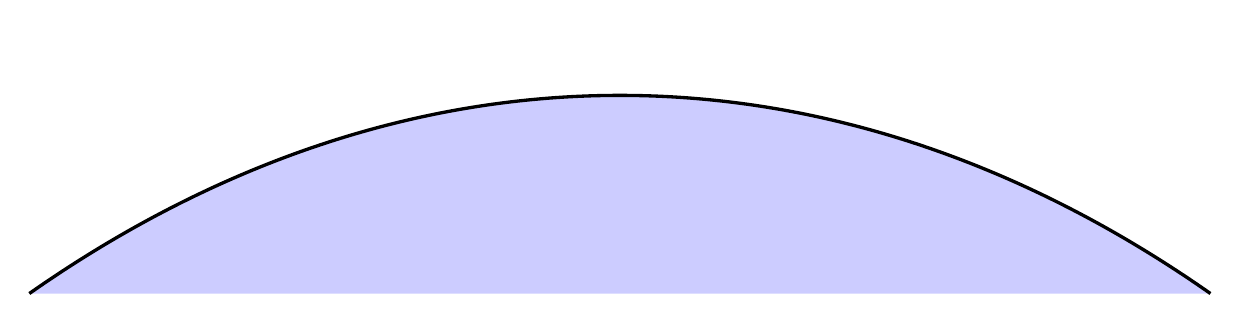
\begin{tikzpicture}
\draw[very thick, draw=black, fill=blue, fill opacity=0.2] (0,0) to [out=35,in=145] (15,0);
\end{tikzpicture}
  	\caption[Pipeline survey]{Scenario}
\end{figure}

\section*{Unmanned Aerial System (UAS)}
In some cases it is necessary to talk about our system as a whole, such that we use it further. The UAS is composed of the following:
\begin{itemize}
	\item Drone
	\item Basestation
	\item Communications
	\item Survey camera
\end{itemize}

\begin{figure}[h!]\label{fig:uas}
	\centering
	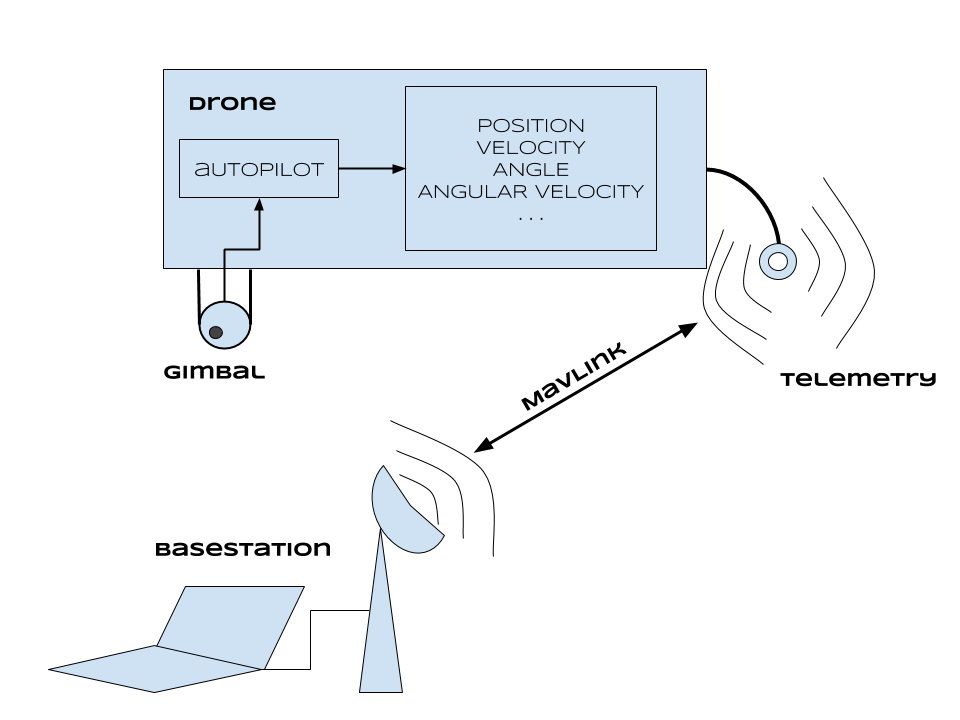
\includegraphics[width=0.7\textwidth]{figures/uas.png}
	\caption{Unmanned Aerial System Overview}
\end{figure}

\section*{Antenna Overview}
The antennas used for the basestation and the drone are different by means of weight and size. The preference of using them is based on the application at hand, thus for:
\begin{itemize}
	\item Basestation - Parabolic (grid) directional antenna 
	\item Drone - Patch directional antenna
\end{itemize}

A parabolic antenna in an antenna that uses a parabolic reflector and a curved surface to direct the radio waves and its main advantage is that it has a high directivity. This type of antennas are able to produce the narrowest beam widths which allow them to have some of the highest gains.

Parabolic antennas, due to their high gain, are intensively used for carry telephone and television signals between nearby cities. In our specific case, it’s possible to use this property to receive the information provided by the thermal camera through the UAS.

Patch antenna, which is the original type of microstrip, is a low profile antenna that can be mounted on a flat surface and it consists in a rectangular sheet of metal. These antennas are very useful because they are very thin and their directivity varies from 5 to 7 dB.

\begin{table}[h!]
\centering
	\begin{tabular}{|c||c|c|}
		\hline
		Parameter & Basestation & Drone\\ \hline\hline
		Type & Parabolic & Patch\\ \hline
		Polarization & Linear & Linear\\ \hline
		Frequency [GHz] & $2.4$ & $2.4$\\ \hline
		Gain [dB] & $24$ & $14$\\ \hline
		HPBW/$H(^{\circ})$ & $14$ & $45$\\ \hline
		HPBW/$V(^{\circ})$ & $10$ & $45$\\ \hline
	\end{tabular}
	\caption{Table of antennas parameters}
	\label{table:1}
\end{table}

\section*{Technical Scenario}
As mentioned before we need to assure the maximum distance of communication possible between the basestation and the drone at a certain working frequency:

\begin{equation*}\label{eq:tech_parameters1} 
 	\begin{cases}
 		d_{max} = 50 km	\\
 		f = 2.4 GHz
 	\end{cases}
\end{equation*}

Computing signal wavelength ($\lambda$) for the working frequency stated above:
\begin{equation*}\label{eq:tech_parameters2}
	\lambda = \frac{c}{f} = \frac{3\cdot 10^{8}}{2.4\cdot 10^{9}} 
	        = 0.125 \text{m}
\end{equation*}

Computing the path loss for a distance of 50 kilometers and the signal wavelength:
\begin{equation*}\label{eq:tech_parameters3}
	L = 20\lg\left (\frac{4\pi d_{max}}{\lambda} \right)
	  = 20\lg\left (\frac{4\pi \cdot 50}{0.125\cdot 10^{-3}} \right)
	  = 134 \text{dB} 
\end{equation*}


Computing the output power of the transmitting antenna of 1 Watt:
\begin{equation*}\label{eq:tech_parameters4}
	P_{TX} = 10\lg\left (\frac{1}{10^{-3}} \right)  
	       = 30 \text{dBm}
\end{equation*}


A simplified link budget omitting some losses of the UAS:
\begin{equation*}\label{eq:tech_parameters5}
	P_{RX} = P_{TX} + G_{TX} + G_{RX} - L  
	       = 30 + 24 + 14 - 134 = -126 \text{dBm}
\end{equation*}


\chapter{Chapter 2 name}\label{ch:ch2label}
Here is chapter 2. If you want to leearn \todo{I think this word is mispelled} more about \LaTeXe{}, have a look at \cite{Madsen2010}, \cite{Oetiker2010} and \cite{Mittelbach2005}.
\missingfigure{We need a figure right here!}


\chapter{Conclusion}\label{ch:conclusion}
In case you have questions, comments, suggestions or have found a bug, please do not hesitate to contact me. You can find my contact details below.
  \begin{center}
    Jesper Kjær Nielsen\\
    \href{mailto: jkn@es.aau.dk}{jkn@es.aau.dk}\\
    \href{http://kom.aau.dk/~jkn}{http://kom.aau.dk/\textasciitilde jkn}\\
    Fredrik Bajers Vej 7\\
    9220 Aalborg Ø
  \end{center}

\printbibliography[heading=bibintoc]
\label{bib:mybiblio}
\appendix
\chapter{Appendix}\label{ch:appAlabel}


\end{document}
